\documentclass[tikz]{standalone}
% Common TikZ styles (built from the user's Graduate Macro Sequence template)
\usepackage{tikz}
\usetikzlibrary{arrows.meta, positioning, calc, decorations.markings}

% Base template styles (user-provided)
\tikzset{
  node style/.style={draw, circle, minimum size=6mm, inner sep=0pt},
  label style/.style={font=\small, sloped, anchor=center},
  arrow style/.style={-{Stealth[length=3mm]}, thick}
}

% Macro-diagram extensions (kept minimal and clean)
\tikzset{
  axis/.style={arrow style},
  curve/.style={thick},
  curve2/.style={thick, dashed},
  helper/.style={thin, dashed},
  dot/.style={circle, fill=black, inner sep=1.2pt},
  lab/.style={font=\small},
  titlelab/.style={font=\small\bfseries},
}

\begin{document}
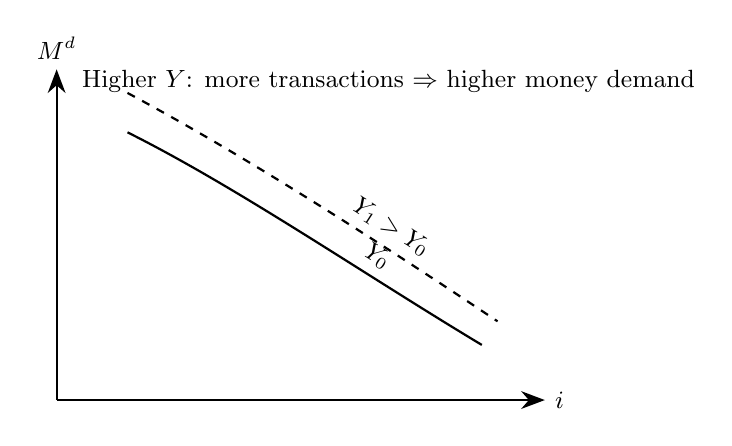
\begin{tikzpicture}[x=1cm,y=1cm]
  \draw[axis] (0,0) -- (6.2,0) node[lab, anchor=west] {$i$};
  \draw[axis] (0,0) -- (0,4.2) node[lab, anchor=south] {$M^d$};

  \draw[curve] (0.9,3.4) .. controls (2.3,2.7) and (3.9,1.6) .. (5.4,0.7)
    node[label style, pos=0.68, above] {$Y_0$};

  \draw[curve2] (0.9,3.9) .. controls (2.4,3.1) and (4.1,2.0) .. (5.6,1.0)
    node[label style, pos=0.68, above] {$Y_1>Y_0$};

  \node[lab, anchor=west] at (0.2,4.05) {Higher $Y$: more transactions $\Rightarrow$ higher money demand};
\end{tikzpicture}
\end{document}
